\documentclass[a4paper]{article}
\usepackage[latin1]{inputenc}
\usepackage{lmodern}
\usepackage[ngerman]{babel}
\usepackage{amsmath}
\usepackage{amssymb}
\usepackage{graphics}
\usepackage{graphicx}
\usepackage{cite}
\usepackage{url}

\title{ImageJ Plugins}
\author{Markus Fischb\"ock (780486)}
\date{BHT Berlin - April 2012}


\begin{document}
\maketitle
\begin{abstract}
Beschrieben ist eine Java Anwendung zur Manipulation von Bildern unter zuhilfenahme der ImageJ Library, sowie
des AWT Frameworks zur Erstellung einer grafischen Oberfl"ache.

\end{abstract}


\newpage
\tableofcontents
\newpage

\section{Einleitung}
Zu erstellen war eine Anwendung, welche unter der Zuhilfenahme der ImageJ Library die Manipulation von Bildern erlaubt. Um die Anwendung komfortabel bedienen zu k"onnen wurde eine grafische Oberfl"ache mit WindowBuilder erstellt. Diese erlaubt es Bilder zu "offnen und manipulierte Bilder abzuspeichern. Eingabeparameter f"ur Plugins sind "uber dedizierte Dialoge einstellbar. Das vorliegende Dokument enth"alt Informationen zu allen Plugins und stellt in kurzem die Funktionsweise einzelner Plugins vor.

\section{Plugins}
\subsection{Channel Remover Plugins}
Das Plugin zum Kanal entfernen bietet dem Benutzer die M"oglichkeit einzelne Farbkan"ale aus dem Eingabebild zu entfernen. Hierzu werden 3 Farbr"aume zur Verf"ugung gestellt, aus denen der Anwender ausw"ahlen kann: RGB, CMY und YUV. Die Funktionsweise der Plugins ist dabei relativ trivial. Es wird "uber alle Pixel des Eingabebildes iteriert und die Farbinformationen der einzelnen Kan"ale extrahiert. Dabei werden die Farbwerte der zu entfernenden Kan"ale auf 0 gesetzt.
Da das Eingabebild zun"achst nur RGB Farbinformationen enth"alt, muss beim entfernen von CMY oder YUV Kan"alen zun"achst intern in den entsprechenden Farbraum konvertiert werden. Hierzu wurden die aus "Ubung 1 erstellten Konverter verwendet, welche erlauben zwischen den einzelnen Farbr"aumen hin und her zu konvertieren. 


\subsection{Brightness Plugin}
Das Plugin zum ver"andern der Helligkeit des Eingabebildes bietet dem Anwender die M"oglichkeit die Helligkeit in unterschiedlichen Farbr"aumen zu ver"andern. Hierzu wurden ebenso wie beim entfernen von Kan"alen die aus "Ubung 1 erstellten Konverter verwendet. Der Benutzer kann hier w"ahlen zwischen RGB, HSV und YUV.
Um eine komfortable Bearbeitungsm"oglichkeit zu bieten, war es notwendig das Ursprungsbild nicht schon beim verschieben des Helligkeitsreglers destruktiv zu bearbeiten, sondern dem Anwender zun"achst eine Vorschau zu bieten. Erst bei der Best"atigung des Dialoges sollte das Ursprungsbild entsprechend transformiert werden. Dies geschieht in der Anwendung unter Zuhilfenahme einer Kopie des Eingabebildes, welches dem Benutzer als Vorschau dient.

Die "Anderungen an der Helligkeit finden in den einzelnen Farbr"aumen auf unterschiedliche Art und Weise statt. Unter Benutzung des RGB Farbraumes werden die Farbwerte alle Kan"ale gleicherma"sen in- oder dekrementiert. YUV und HSV bieten f"ur die Helligkeitsregelung dedizierte Kan"ale, welche das "andern der Helligkeit basierend auf einem einzelnen Wert erlauben. Beim YUV Farbraum ist dazu der Y-Parameter (Luminanz) zust"andig. Beim HSV Farbraum reicht es aus, den V-Parameter entsprechend zu ver"andern. 

Auff"allig ist, dass beim RGB Farbraum die besten Ergebnisse erzielt werden. Eine "Anderung der Helligkeit im HSV oder YUV Farbraum unter Verwendung des gleichen Eingabeparameters f"ur die Helligkeit f"uhrt schnell zum Verlust von Farbinformationen. Dies liegt m"oglicherweise unter anderem an Rundungsfehlern die bei der Konvertierung in die entsprechenden Farbr"aume auftreten.


\subsection{Skalierung}
Das Plugin zur Skalierung bietet dem Anwender zun"achst die M"oglichkeit die Ausgabegr"o"se des Bildes anhand zweier sogenannter ``Spinner'' widgets einzustellen. Ein zus"atzlicher Schalter erlaubt es ausserdem, die Regler so miteinander zu verbinden, dass die Proportionen des Eingabebildes erhalten bleiben. Weiter wird dem Anwender angeboten den Algorithmus, welcher zur Skalierung verwendet wird zu bestimmen. Hier werden 2 Verfahren angeboten, welche im folgenden kurz erkl"art werden.

\subsubsection{Nearest Neighbor}
Bei der Skalierung unter Verwendung des Nearest Neighbor Verfahrens, wird zun"achst die Position des Ausgabepixels ermittelt. Dies geschieht unter Verwendung folgender Gleichungen:

\begin{equation}
\label{EQ_findPoint}
	x = \frac{x' (w - 1)}{(w' - 1)} \hspace{2 cm} y = \frac{y' (h - 1)}{(h' - 1)}
\end{equation}

Die Farbinformation des hiermit berechneten Punktes wird nun durch Runden der Werte und Extraktion aus dem Quellbild ermittelt. Das Verfahren selbst ist sehr schnell, beinhaltet aber den Nachteil, dass bei Skalierung mit hohen Gr"o"senunterschieden Artefakte auftreten.


\subsubsection{Bilinear}
Bei der bilineraren Interpolation wird die Position des Augabepixels zun"achst so berechnet, wie das auch beim Nearest Neighbor Verfahren der Fall ist. Hierbei wird der Farbwert des neuen Pixels allerdings nicht durch Runden der resultierenden Werte ermittelt, sondern es wird zwischen 4 Punkten interpoliert. Da das Augabepixels irgendwo zwischen 4 Eingabepixeln liegt, muss der Farbwert anteilig berechent werden. Dabei werden zun"achst in horizontaler Richtung die Farbwerte ermittelt und deren Resultate nochmals zwischen den beiden vertikalen Pixeln anteilig berechnet.
Das Verh"altnis der Farbwerte zueinander wird dabei "uber folgende Gleichung ermittelt:

\begin{equation}
\label{EQ_ratio}
	n_\text{x} = x - \lfloor x \rfloor \hspace{2 cm} n_\text{y} = y - \lfloor y \rfloor
\end{equation}
Ausgehend von diesen Verh"altnissen, werden die horizontalen Farbwerte ermittelt:

\begin{equation}
\label{EQ_horizontal_interpolation}
	\begin{aligned}
	& a = (1 - n_\text{x}) \cdot I(\lfloor x \rfloor, \lfloor y \rfloor) + n_\text{x} \cdot I (\lceil x \rceil, \lceil y \rceil)\\
	& b = (1 - n_\text{x}) \cdot I(\lfloor x \rfloor, \lceil y \rceil) + n_\text{x} \cdot I (\lceil x \rceil, \lceil y \rceil)
	\end{aligned}
\end{equation}
Anschlie"send flie"sen die resultierenden Werte in die vertikale Interpolation mit ein:
\begin{equation}
\label{EQ_vertical_interpolation}
	p = (1 - n_\text{y} ) \cdot a + n_\text{y} \cdot b
\end{equation}

\newpage
\subsection{Histogramm}
Das Histogram Plugin ermittelt die Helligkeitswerte des Eingabebildes und gibt das resultierende Histogramm des Bildes in einem Dialog wieder. Zur Erstellung des Graphen wurde auf die Library JFreeChart zur"uckgegriffen, welche f"ur das erstellen von Histogrammen eigene Methoden anbietet. Der Benutzer hat bei der Erstellung des Histogramms die M"oglichkeit dies, f"ur unterschiedliche ausw"ahlbare Farbr"aume zu tun. Angeboten werden hierf"ur RGB, YUV und HSV. Zwar wird die Bibliothek JFreeChart unter der LGPL angeboten, jedoch ist eine ausf"uhrliche Dokumentation leider nur gegen Bezahlung erh"altlich, was zu Einschr"ankungen in der Erstellung des Diagramms f"uhrte. Geplant war hierf"ur eigentlich alle Kan"ale separat anzuzeigen. Per Default wird im Hintergrund auch ein Schatten der Kurve gezeichnet, was eher st"orend wirkt, dies konnte jedoch aufgrund mangelnder Dokumentation ebenfalls nicht angepasst werden.

\begin{figure}[htp]
\centering
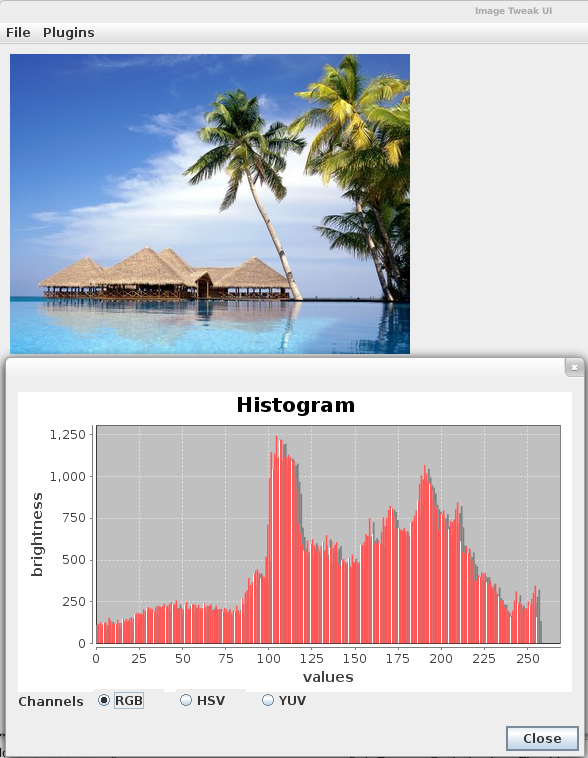
\includegraphics[scale=0.50]{histogram.png}
\caption{ImageTweak UI - RGB Histogram}
\label{ImageTweak UI - RGB Histogram}
\end{figure}

\subsection{Blur Filter}
Der Blur Filters wurde mit Hilfe einer Konvolutionsmatrix implementiert. Hierbei wird "uber jedes Pixel im Bild iteriert und der neue Farbwert als Mittel des aktuellen Pixels und aller seiner Nachbarn berechnet. Entscheidend ist dabei, nicht "uber die Grenzen des vorhandenen Bildes zuzugreifen. Ein erster Ansatz mit 2 Schleifen, welche in X und Y Richtung iterieren war von Fehlern gepr"agt. Nach einer "Uberarbeitung des Algorithmus und der Begrenzung auf eine Richtung - was vollkommen ausreichend ist - konnten diese Fehler beseitigt werden.

\section{Erweiterungen}
Aufgrund von Zeitmangel war es mir nicht m"oglich zus"atzliche Aufgabenstellungen zu bearbeiten. Jedoch war bei der Planung ein zentraler Punkt, eine Anwendung mit einer grafischen Oberfl"ache zu erstellen. Zwar bot ImageJ hierf"ur rudiment"are M"oglichkeiten um einfache Dialoge zu erstellen, der Fokus lag aber in meiner Implementierung darauf alles in einer komfortabel zu bedienenden GUI darzustellen.
Aufgrund dieser Entscheidung zu Beginn der Aufgabe, fiel das Augenmerk schnell auf das Eclipse Plugin ``Window Builder'' mit dem per WYSIWYG Editor auf schnelle und unkomplizierte Weise grafische Oberfl"achen erzeugt werden k"onnen. 
Der Mehraufwand der Entwicklung eines GUI stelle sich allerdings im Laufe der Bearbeitung der Aufgabe als sehr zeitraubend heraus, woraus ich f"ur kommende Aufgaben schlie"se, dass es vern"unftiger ist n"aher an der eigentlichen Aufgabenstellung zu arbeiten.

\newpage

\bibliography{cg-quellen.bib}{}
\bibliographystyle{gerplain}

\end{document}
